\chapter[Chapter 1: Introduction]{Introduction}

\section{Background}

With the increased popularity of online classes, as well as a rise in enrollment in foundational courses for engineering, students need an interactive learning tool that guides them through homework problems when assistance from a professor, teaching assistant, or another student is unavailable. This is especially important in an environment where students with diverse schedules must attend class (i.e. managing work and class or studying abroad). Increased retention and student success in any course requires good communication and interaction among students and instructors.  However, the expectation of access to instructors at any time is unrealistic with the constriction in teaching staff because of reductions in funding.

I am going to develop a \gls{cita} for the introductory electricity and magnetism class at Purdue University (PHYS 24100 and PHYS 24100D) that will be available to guide students through homework problems at any time. The most often heard statement from students attempting the homework or practice exams is, ``I don’t even know where to begin.'' With \gls{cita} we propose to design an interactive component for every problem that will guide the student through a focused strategy for problem solving. \gls{cita} will guide students through problems in such a way as to develop critical thinking and problem solving skills with a thorough understanding of the physical concepts.

Most computerized homework systems only provide a ``correct'' or ``incorrect'' response to a student’s answers. If a student receives the ``incorrect'' message, there is no explanation as to why their logic was wrong and no rarely any hints on how to proceed from their current analysis. At the very most, there is a link to a section in the online textbook that is often too general for the specific problem at hand. The student either has to email an instructor, wait for recitation later in the week, or seek special appointments with instructors. The learning process is interrupted as the student waits for what often is simple guidance. Our goal is to design, develop, implement, and analyze an online program that is available at any time to provide focused guidance to help students acquire critical thinking skills and develop a problem solving strategy.

\section{Overview of PHYS 24100 at Purdue}

PHYS 24100 is the introductory electricity and magnetism course for engineering majors at Purdue University. It is generally taken after students complete PHYS 17200 - the introductory mechanics course. The mechanics course is currently taught using the Matter and Interactions[CITATION NEEDED] textbook by Sherwood and Chabay. PHYS 24100 is a prerequisite for many of the intermediate engineering courses at Purdue University.

\begin{figure}[hb]
	\centering
	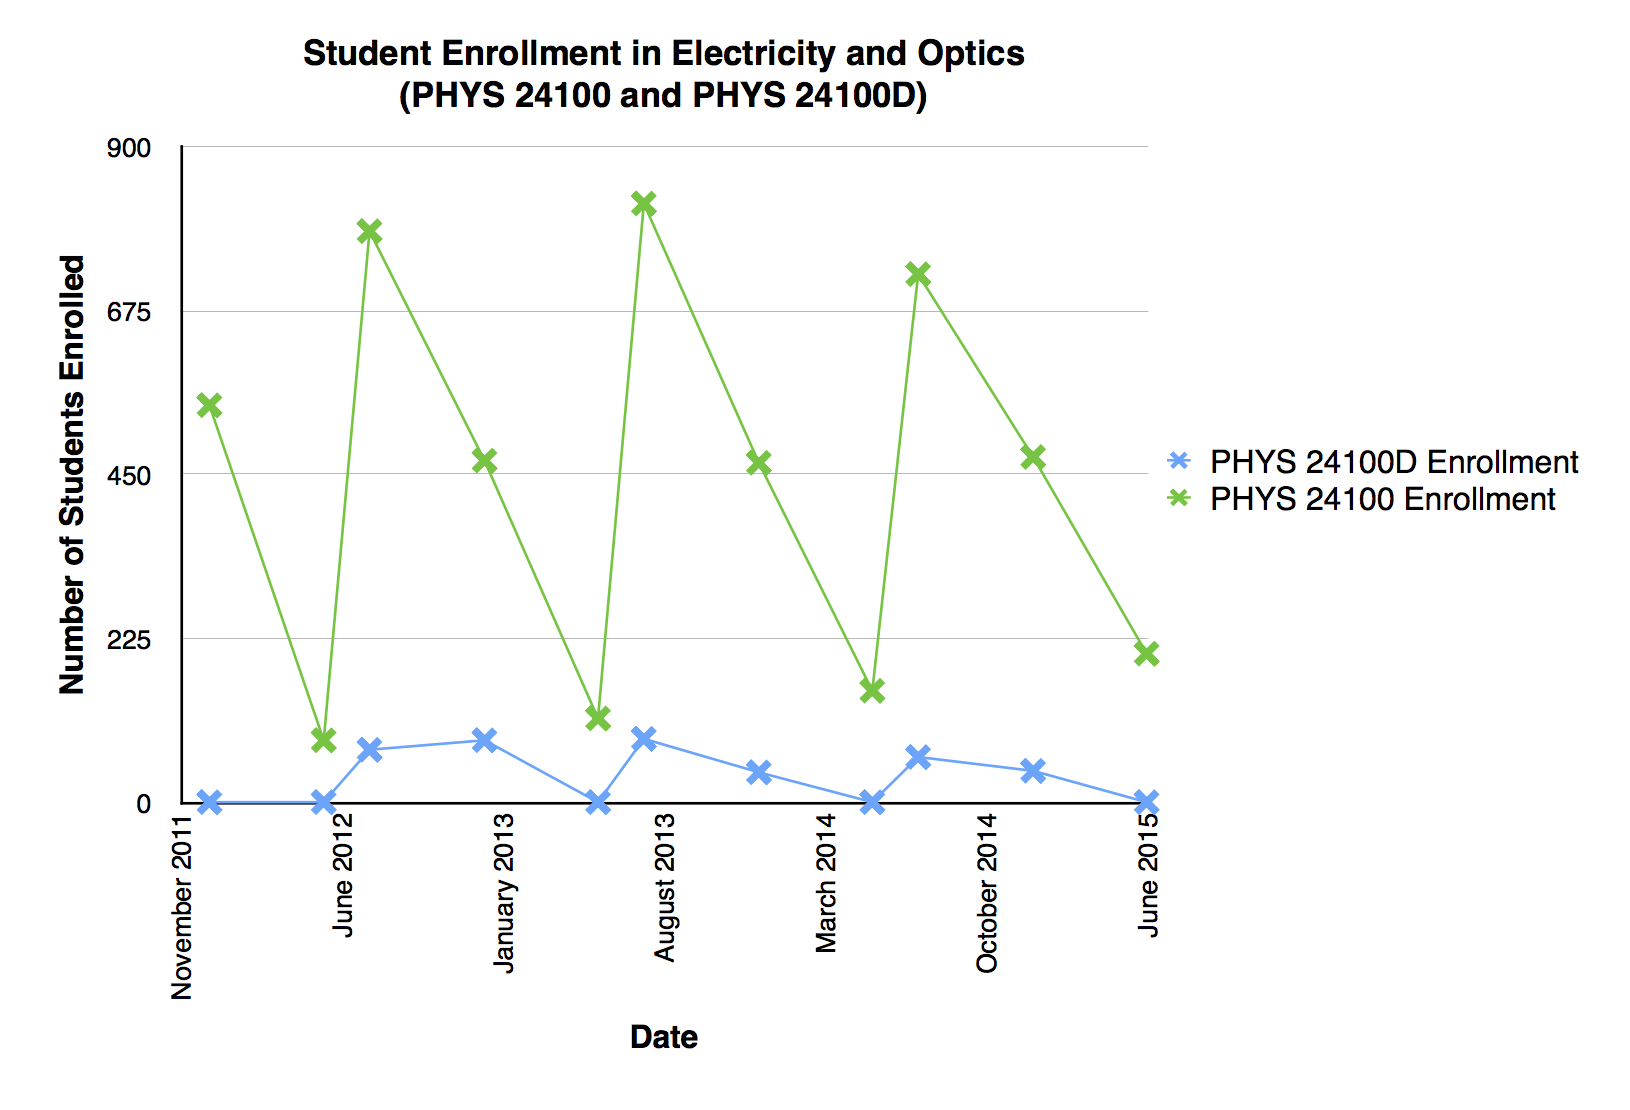
\includegraphics[width=6in]{img/chapter1/enrollment}
	\caption[Enrollment in Electricity and Optics]{Enrollment in Electricity and Optics}
\end{figure}

This is another figure.

\begin{figure}[hb]
	\centering
	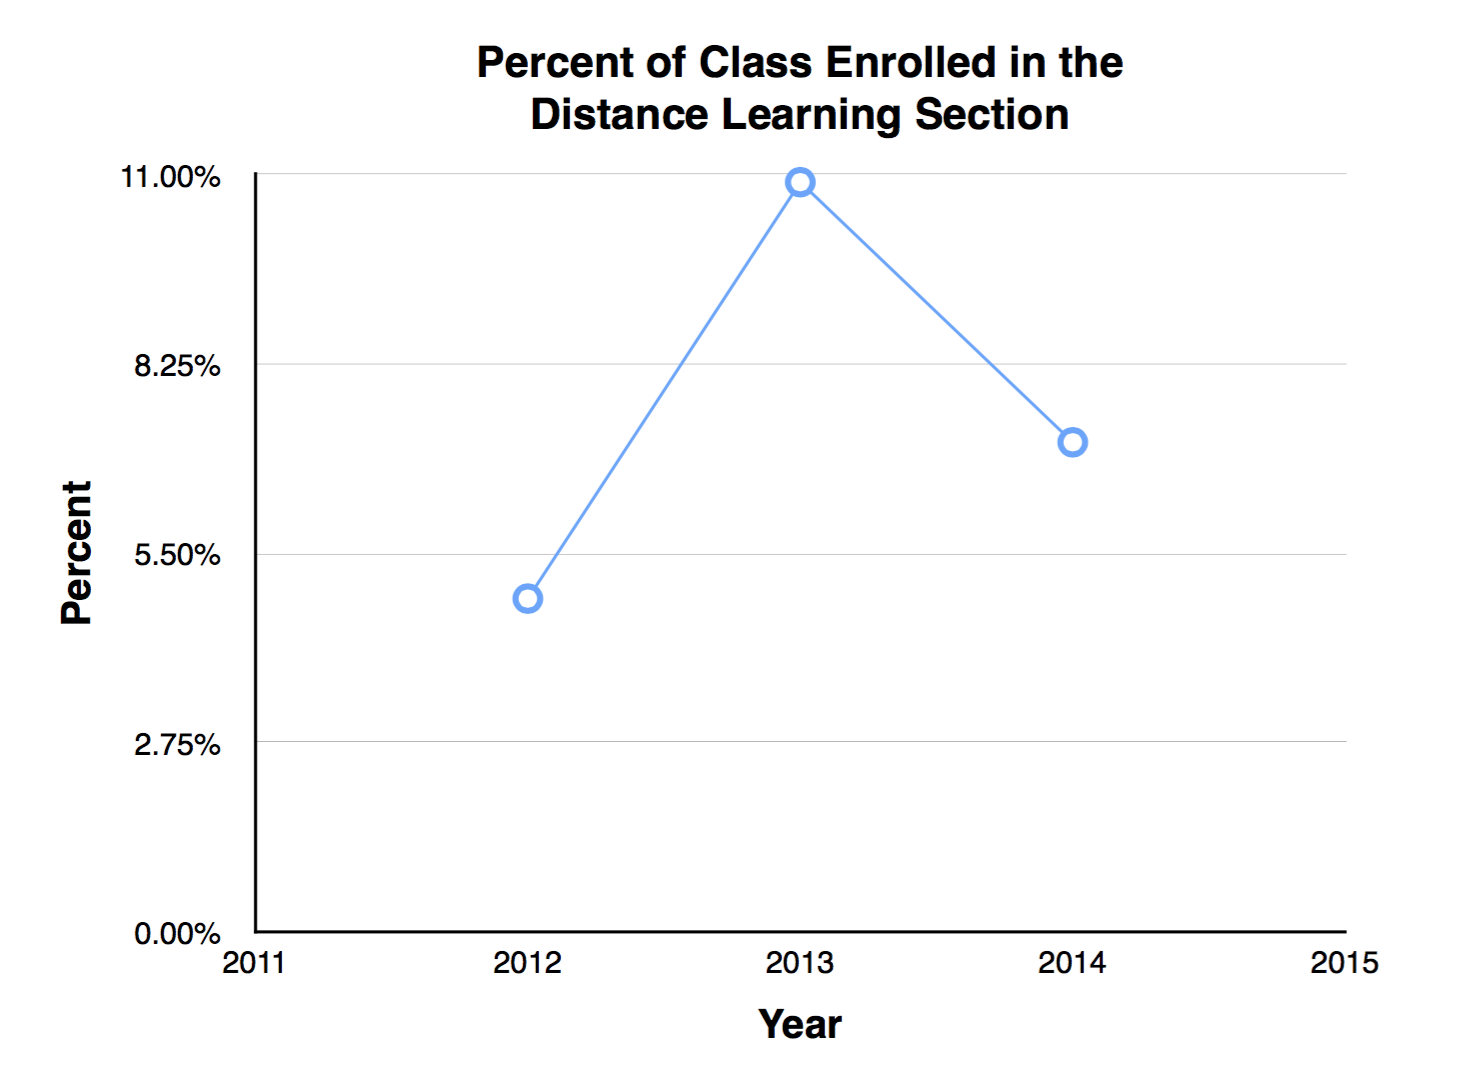
\includegraphics[width=6in]{img/chapter1/percent}
	\caption[Percent of Students in Distance Learning Class]{Percent of Students in Distance Learning Class}
\end{figure}

\section{Overview of CHIP at Purdue}

In the Physics department, we have access to thousands of problems from several different textbooks from several publishers through our computerized homework system – \gls{chip}. Very few of these problems have an interactive approach to problem solving. However this semester, we received very positive student feedback on these

\subsection{Strengths}

The \gls{chip} program at Purdue is a well established system that has over a decade of in-the-field use. One of its biggest advantages is that it has no ties to any external companies or organizations. The faculty at Purdue is free to update or modify the source code as they wish. All of the \gls{chip} servers are maintained on Purdue University campus in the physics building by our own IT support team.

\gls{chip} has a dedicated staff of experts that run and maintain the system. This faculty works for Purdue University, so there is no conflict of interest outsourcing this job to other companies.

\gls{chip} has a well developed database of problems from a variety of textbooks. We have permission to use. Additionally, \gls{chip} keeps a secure archive of scores from previous semesters.

\gls{chip} already has the framework in place to collect statistics on student performance during the semester. On a basic level, it is capable of recording student scores in a variety of assignments. However, it can also perform a basic statistical.

\gls{chip} offers a few advantages to students as well as faculty. \gls{chip} comes at no extra cost to students - students only need to buy the course textbook rather than a course textbook and site license. \gls{chip} has a mature gradebook that students can use to get feedback on assignments; if they are enrolled in an online course, this feedback is instantaneous because the entire system is self-contained. Additionally, when students ask questions or send error reports, they are talking directly with a course instructor rather than a secondary source. This facilitates communication and solves problems in a more timely fashion.

\subsection{Weaknesses}

Although \gls{chip} has a successful history at Purdue, it is not without its problems. The \gls{chip} program was coded in the late 90s and early 2000s. Thus, while the graphical user interface (GUI) was revolutionary at one time, it has begun to show its age. The overall look and layout of \gls{chip} has not kept up with modern devices. Specifically, \gls{chip} buttons and menus do not render well on small screens like cell phones, tablets, and netbooks.

\gls{chip} has a lot of underutilized features. For example, different statistical analysis tools are available on the system, but they are rarely used due to the fact that they are either hard to find or require a learning curve.

Interactive tutorials have been implemented on only 29 out of 139 homework problems (about 20.9\% of the problems). interactive examples (e.g. ``Thank you for the help section in this problem! It was very well written and helped me figure out the problem and (hopefully) similar ones in the future!'' and ``These really help get started and grasp a main idea for the homework.''). This suggests that the interactive feature should be expanded to assist the thousands of students enrolled annually in the course. This is especially important in light of the increased enrollment in the distance learning PHYS 241D. An example of the approach is given in Appendix A for the \gls{chip} problem that received student feedbackThese tutorials are certainly useful for solving the specific problem at hand, but they do little to inspire creativity and discussion in the classroom.

\section{Statement of Purpose}

We want to develop an online \gls{cita} for the second semester of introductory physics. This tutorial would be available to guide students through problem solving at any time. The most often heard statement to our teaching assistants for PHYS 241D and 241 from students attempting the homework or practice exams is, ``I don’t even know where to begin.''  With \gls{cita} we propose to design an interactive component for each individual problem that will guide the student through a focused strategy for problem solving. \gls{cita} will guide students through problems in such a way as to develop critical thinking and problem solving skills with a thorough understanding of the physical concepts.

Development and implementation of \gls{cita} on \gls{chip} requires work to

\begin{enumerate}
\item Update graphical user interfaces (GUIs) to maximize potential impact
\item Develop and implement \gls{cita} guides for every problem
\item Include interactive graphics for interactive learning of basic concepts
\item Update, improve and implement the graphical tools for learning assessment data visualization for instructors
\end{enumerate}

\section{Problem Statement}

What is revolutionary about our system is the immersive structure of the tutorials. Students are encouraged to think about problems in different ways as they traverse different paths to obtaining a solution. Thus, in our research, we pay special attention to the structure of this system.

\begin{enumerate}
\item How does the branching structure of our interactive examples influence student problem solving?
\item What do students think about our interactive tutorials?
\end{enumerate}